Our program produced the correct results on everything we tested. Note that we don't keep track of everything in terms of $\pi$s, so they appear as floating point numbers in our solutions.

\begin{figure}[H]
	\raggedright
	Our output: \\
	\begin{verbatim}
Input:    log(-1.000+Z)^-1.000
Deriv:
-1.000*(log(-1.000+Z)^-2.000*(-1.000+Z)^-1.000)
Zeros:    List()
Singular: List(-2.000+Z)
Branch:   List(-1.000+Z)
Cluster:  List()
\end{verbatim} \vspace{7pt}
	WolframAlpha output:\\
	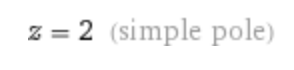
\includegraphics[width=0.4\columnwidth]{images/wpoles1}
	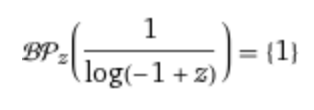
\includegraphics[width=0.4\columnwidth]{images/wbranch1}
	\caption{Our output and WolframAlpha's for $1/log(z-1)$.}
	\label{fig:singEx1}
\end{figure}
Our program outputs zeros, singular points, branch points, and cluster points in terms of equations that should equal zero. This means that our program found a singular point at $z=2$ and a branch point at $z=1$, which is the same as the results from when we did it manually in Section~\ref{sec:expressions}, and the same as WolframAlpha's results.

\begin{figure}[H]
	\raggedright
	Our output: \\
	\begin{verbatim}
Input:    cos(Z^-1.000)^-1.000
Deriv:    -1*(cos(Z^-1)^-2*Z^-2*sin(Z^-1))
Zeros:    List()
Singular:
List(-1*((1.571+3.142*n1)^-1*(e^(-6.283i*n2)))+Z)
Branch:   List()
Cluster:  List(Z)
	\end{verbatim} \vspace{7pt}
	WolframAlpha output:\\
	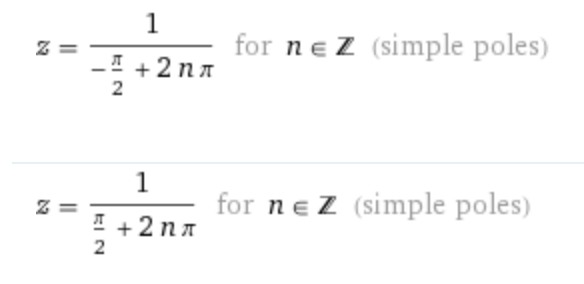
\includegraphics[width=0.6\columnwidth]{images/wpoles2}
	\caption{Our output and WolframAlpha's for $1/cos(1/z)$, some decimals have been truncated for brevity.}
	\label{fig:singEx2}
\end{figure}
While it may not be obvious from the start, our output, WolframAlpha's, and what we worked out in Section~\ref{sec:expressions} are equivalent, with the exception that WolframAlpha doesn't report cluster points. The $e^{-6.283in_2}$ exists because we don't have a rule to simplify it to $1$.

\begin{figure}[H]
	\raggedright
	Our output: \\
	\begin{verbatim}
Input:    sin(sin(Z)^-1.000)^-1.000
Deriv:
sin(sin(Z)^-1)^-2*sin(Z)^-2*cos(sin(Z)^-1)*cos(Z)
Zeros:    List()
Singular:
List(-1*asin(0.318*((e^(-6.283i*n2))*n1^-1))+
-6.283*n3+Z)
Branch:   List()
Cluster:  List(-3.142*n5+-6.283*n3+Z)
	\end{verbatim} \vspace{7pt}
	WolframAlpha output:\\
	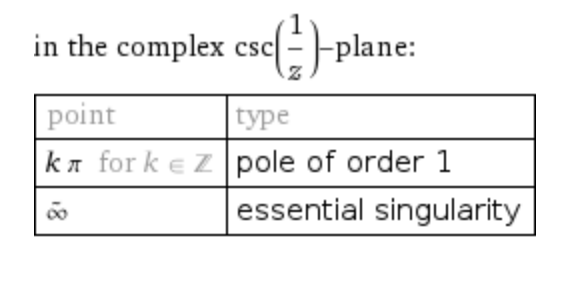
\includegraphics[width=0.6\columnwidth]{images/wpoles3}
	\caption{Our output and WolframAlpha's for $1/sin(1/sin(z))$, some decimals have been truncated for brevity. Note that $1/\pi=0.318.$}
	\label{fig:singEx3}
\end{figure}
Our output is once again equivalent to what we derived in Section~\ref{sec:expressions}, with the exception that there are many more quantifiers (the $n_i$'s), that haven't been simplified out. WolframAlpha technically outputs the same thing, but it fails to solve the equations and instead outputs the answer in terms of the $csc(z)$-plane, which makes its results harder to interpret and use. It also doesn't identify cluster points.
